\documentclass{article}


\usepackage[T1]{fontenc}
\usepackage[short]{optidef}
\usepackage[caption=false,font=footnotesize]{subfig}
\usepackage{adjustbox}
\usepackage{algorithm}
\usepackage{algpseudocode}
\usepackage{amsfonts}
\usepackage{amsmath}
\usepackage{amssymb}
\usepackage{amsthm}
\usepackage{cite}
\usepackage{framed}
\usepackage{fullpage}
\usepackage{mathtools}
\usepackage{microtype}
\usepackage{multirow}
\usepackage{pdfpages}
\usepackage{pgfplots}
\usepackage{siunitx}
\usepackage{xr-hyper}
\usepackage{hyperref}

\externaldocument[M-]{../main}

\DeclareSIUnit{\belm}{Bm}
\DeclareSIUnit{\dBm}{\deci\belm}
\DeclareSIUnit{\beli}{Bi}
\DeclareSIUnit{\dBi}{\deci\beli}

\newcounter{reviewer}
\setcounter{reviewer}{0}
\newcounter{point}[reviewer]
\setcounter{point}{0}
\newcounter{response}[reviewer]
\setcounter{response}{0}

\let\svbibcite\bibcite
\def\bibcite#1#2{\svbibcite{#1}{R#2}}
\makeatletter
\let\svbiblabel\@biblabel
\def\@biblabel#1{\svbiblabel{R#1}}
\makeatother

\renewcommand{\theequation}
	{E\arabic{equation}}

\renewcommand{\thefigure}
	{F\arabic{figure}}

\renewcommand{\thetable}
	{T\arabic{table}}

\renewcommand{\thealgorithm}
	{A\arabic{algorithm}}

\newcommand{\reviewer}
	{\stepcounter{reviewer} \bigskip \hrule \section*{Reviewer \thereviewer}}

\renewcommand{\thepoint}
	{\thereviewer.\arabic{point}}

\renewcommand{\theresponse}
	{\thereviewer.\arabic{response}}

\newenvironment{point}
	{\refstepcounter{point} \bigskip \noindent {\textbf{Comment~\thepoint} } ---\ \itshape}
	{\par}

\newenvironment{response}
	{\refstepcounter{response} \medskip \noindent \textbf{Response:}\ }
	{\medskip}


\begin{document}
	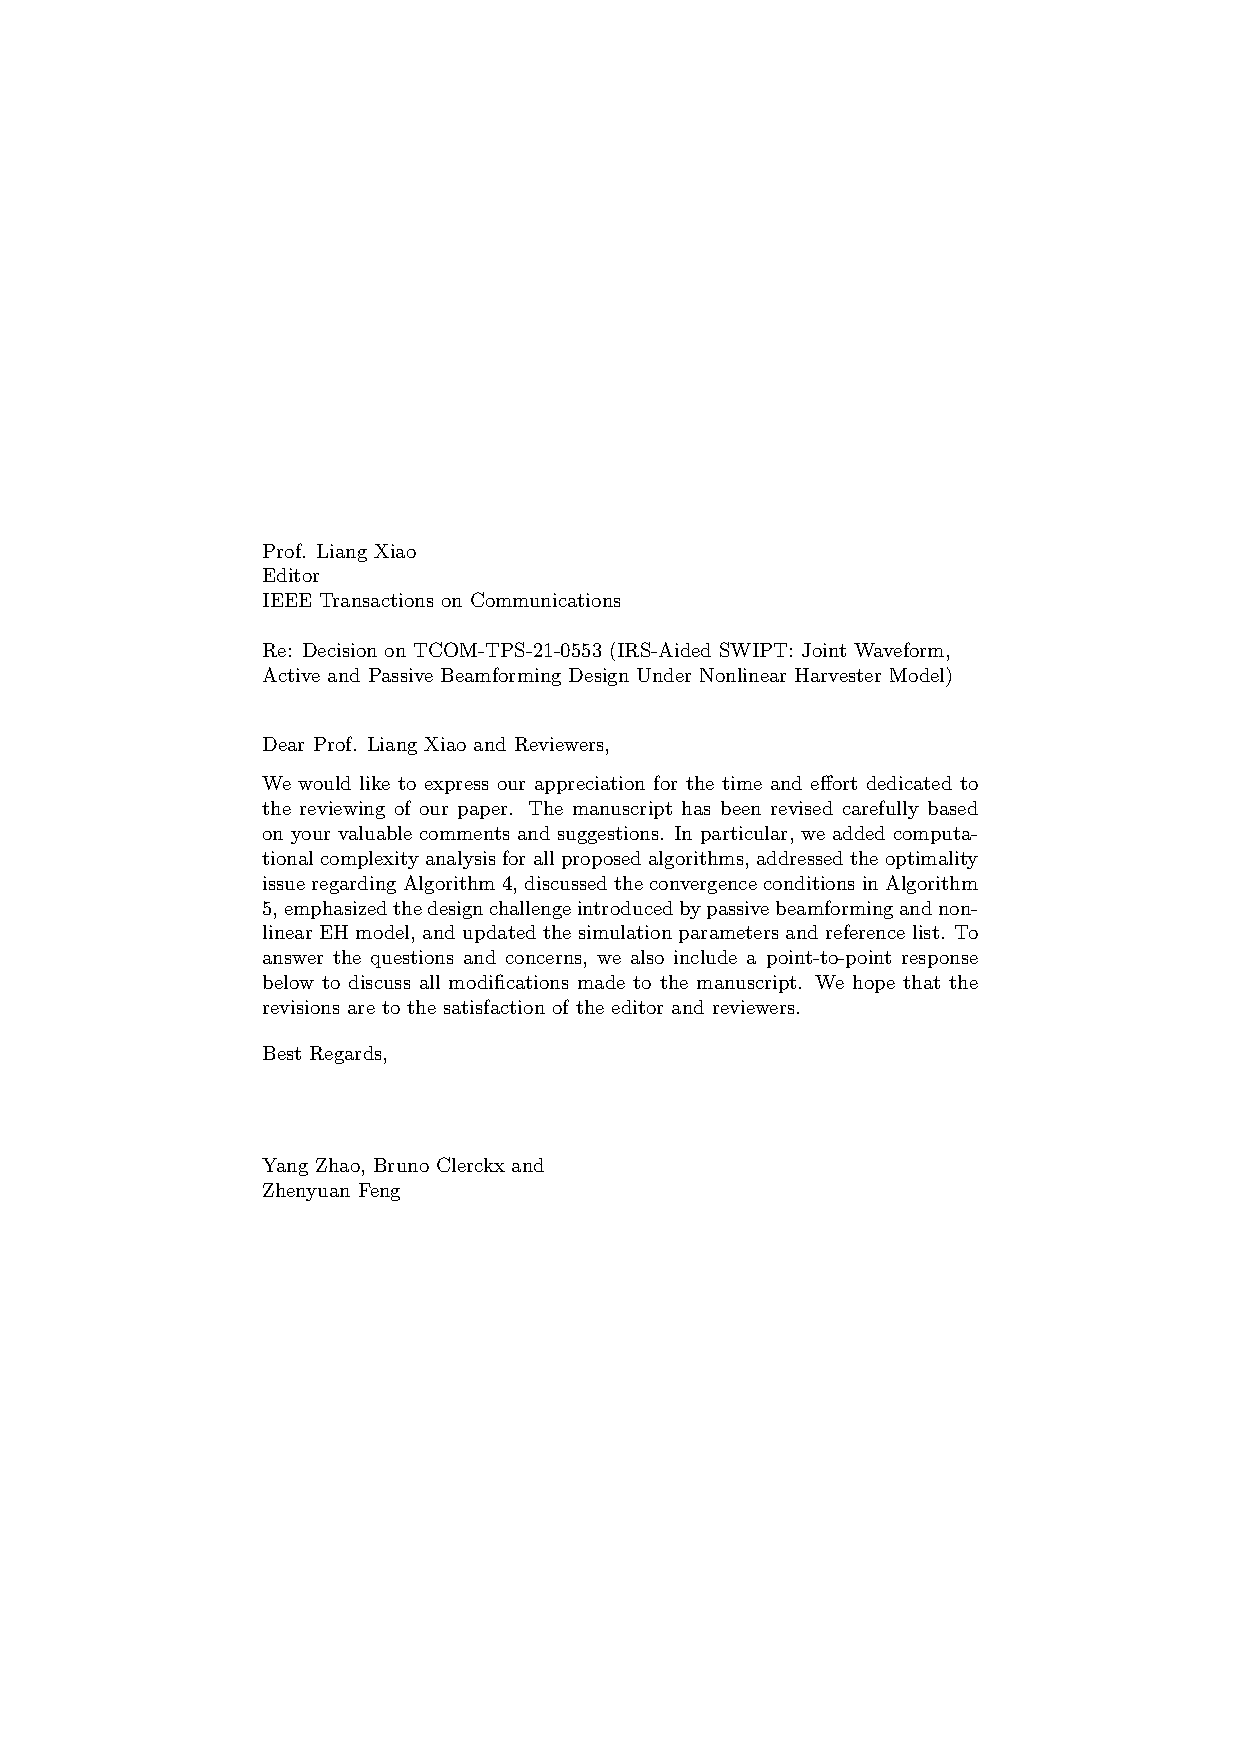
\includepdf{letter_2.pdf}

	\begin{reviewer}
		\begin{point}
			As this paper proposed a BCD-based algorithm and LC-BCD algorithm, it could be better if the authors can further discuss the complexity and provide some measurements or some simulation results.
		\end{point}

		\begin{response}
			We appreciate your suggestion and agree that complexity analysis is necessary in algorithm evaluation.

			For SCA Algorithm~\ref{M-al:sca}, in the previous manuscript, we applied SCA on $t_{\mathrm{I},0} t_{\mathrm{P},0}$ at iteration $i$ as
			\begin{align}
				t_{\mathrm{I},0}^{(i)} t_{\mathrm{P},0}^{(i)}
				& = \frac{1}{4}(t_{\mathrm{I},0}^{(i)} + t_{\mathrm{P},0}^{(i)})^2 - \frac{1}{4}(t_{\mathrm{I},0}^{(i)} - t_{\mathrm{P},0}^{(i)})^2\nonumber\\
				& \ge \frac{1}{2}(t_{\mathrm{I},0}^{(i)} + t_{\mathrm{P},0}^{(i)})(t_{\mathrm{I},0}^{(i-1)} + t_{\mathrm{P},0}^{(i-1)}) - \frac{1}{4}(t_{\mathrm{I},0}^{(i-1)} + t_{\mathrm{P},0}^{(i-1)})^2 - \frac{1}{4}(t_{\mathrm{I},0}^{(i)} - t_{\mathrm{P},0}^{(i)})^2,
			\end{align}
			which is generally feasible and widely adopted when $t_{\mathrm{I},0}$ and $t_{\mathrm{P},0}$ are variables. Hence, we claimed Algorithm~\ref{M-al:sca} ``is not a Semidefinite Programming (SDP) due to the quadratic objective function \eqref{M-eq:z_irs_approx}''. During revision, we realized that $t_{\mathrm{I/P},0}=\mathrm{tr}(\boldsymbol{C}_{\mathrm{I/P},0}\boldsymbol{\Phi})$ are essentially linear real expressions related to optimization variable $\boldsymbol{\Phi}$, and the SCA can be further reduced to
			\begin{equation}
				t_{\mathrm{I},0}^{(i)} t_{\mathrm{P},0}^{(i)} \ge t_{\mathrm{I},0}^{(i)} t_{\mathrm{P},0}^{(i-1)} + t_{\mathrm{P},0}^{(i)} t_{\mathrm{I},0}^{(i-1)} - t_{\mathrm{I},0}^{(i-1)} t_{\mathrm{P},0}^{(i-1)}.
			\end{equation}
			Therefore, the quadratic term in the objective function \eqref{M-eq:z_irs_approx} is eliminated and the updated problem~\ref{M-op:irs} is indeed an SDP. Given a solution accuracy $\epsilon_{\mathrm{IPM}}$ for the interior-point method, the computational complexity of Algorithm~\ref{M-al:sca} is $\mathcal{O}\left(I_{\mathrm{SCA}}(L+2)^4 (L+1)^{0.5} \log(\epsilon_{\mathrm{IPM}}^{-1})\right)$, where $I_{\mathrm{SCA}}$ denotes the number of SCA iterations \cite{M-Luo2010}. We have revised the manuscript as follows.
			\begin{framed}
				The passive beamforming design is summarized in the SCA Algorithm~\ref{M-al:sca}, where the relaxed problem \eqref{M-ob:irs}--\eqref{M-co:irs_sd} involves a $(L+1)$-order positive semi-definite matrix variable and $(L+2)$ linear constraints. Given a solution accuracy $\epsilon_{\mathrm{IPM}}$ for the interior-point method, the computational complexity of Algorithm~\ref{M-al:sca} is $\mathcal{O}\left(I_{\mathrm{SCA}}(L+2)^4 (L+1)^{0.5} \log(\epsilon_{\mathrm{IPM}}^{-1})\right)$, where $I_{\mathrm{SCA}}$ denotes the number of SCA iterations \cite{M-Luo2010}.
			\end{framed}

			For GP Algorithm~\ref{M-al:gp}, the computational complexity is exponential w.r.t. the number of subbands \cite{M-Chiang2005}.
			\begin{framed}
				The joint waveform amplitude and splitting ratio design is summarized in the GP Algorithm~\ref{M-al:gp}, which achieves local optimality at the cost of exponential computational complexity \cite{M-Chiang2005}.
			\end{framed}

			For M-SCA Algorithm~\ref{M-al:m_sca}, each optimization problem involved is an SDP with $(L+1)$ variables and linear constraints, and the computational complexity is $\mathcal{O}\left(I_{\mathrm{M-SCA}}(L+1)^{4.5} \log(\epsilon_{\mathrm{IPM}}^{-1})\right)$ where $I_{\mathrm{M-SCA}}$ denotes the number of M-SCA iterations.
			\begin{framed}
				Compared with Algorithm~\ref{M-al:sca}, the rate constraint \eqref{M-co:irs_rate} is dropped and each SDP in Algorithm~\ref{M-al:m_sca} involves $(L+1)$ linear constraints. Given a solution accuracy $\epsilon_{\mathrm{IPM}}$ for the interior-point method, the computational complexity of Algorithm~\ref{M-al:m_sca} is $\mathcal{O}\left(I_{\mathrm{M-SCA}}(L+1)^{4.5} \log(\epsilon_{\mathrm{IPM}}^{-1})\right)$, where $I_{\mathrm{M-SCA}}$ denotes the number of M-SCA iterations \cite{M-Luo2010}. Note that $I_{\mathrm{M-SCA}}=1$ for the WIT point since the current expression is dropped and no SCA is involved.
			\end{framed}

			For BCD Algorithm~\ref{M-al:bcd}, since Algorithm~\ref{M-al:gp} is involved per iteration, the computational complexity is exponential w.r.t. the number of subbands.
			\begin{framed}
				The steps are summarized in the BCD Algorithm~\ref{M-al:bcd}, which achieves local optimality with exponential computational complexity. [TODO]
			\end{framed}

			For LC-BCD Algorithm~\ref{M-al:lc_bcd}, both waveform and active beamforming are obtained in closed form, and the computational complexity of Algorithm~\ref{M-al:lc_bcd} is $\mathcal{O}\left(I_{\mathrm{LC-BCD}}I_{\mathrm{M-SCA}}(L+1)^{4.5} \log(\epsilon_{\mathrm{IPM}}^{-1})\right)$, where $I_{\mathrm{LC-BCD}}$ denotes the number of LC-BCD iterations \cite{M-Luo2010}.
			\begin{framed}
				Given a solution accuracy $\epsilon_{\mathrm{IPM}}$ for the interior-point method, the computational complexity of Algorithm~\ref{M-al:lc_bcd} is $\mathcal{O}\left(I_{\mathrm{LC-BCD}}I_{\mathrm{M-SCA}}(L+1)^{4.5} \log(\epsilon_{\mathrm{IPM}}^{-1})\right)$, where $I_{\mathrm{LC-BCD}}$ denotes the number of LC-BCD iterations \cite{M-Luo2010}.
			\end{framed}
		\end{response}

		\begin{point}
			Since this paper focused on IRS-aided SWIPT systems, it could be better if the authors can further enrich the survey part to make the paper more comprehensive. In particular, some papers have considered this kind of problem from a different aspect such as \cite{Xu2021}. It is kindly suggested to briefly discuss the main difference between \cite{Xu2021} and the problem considered in this paper.
		\end{point}

		\begin{response}
			Thank you for sharing this paper. Instead of optimizing the phase shift of each IRS element, it tailored a tile-based two-stage optimization framework for large-scale IRS to enable a flexible performance-complexity tradeoff. The model also adapts well to practical IRS models accounting AoA and AoD. In contrast, our paper is more focused on waveform design and rate-energy tradeoff for one SWIPT user with practical co-located information decoder and energy harvester. We have updated the manuscript as follows.
			\begin{framed}
				In \cite{Xu2021}, the authors proposed a scalable resource allocation framework for SWIPT systems involving large-scale IRS, where the reflectors are grouped into tiles and the optimization process is divided into an offline mode-design stage and an online mode-selection stage to reduce overall complexity. It was concluded that the tile-based two-stage algorithm not only enables a flexible balance between performance and complexity but also adapts well to the physics-based IRS model accounting AoA and AoD. To the best of our knowledge, all existing IRS-aided SWIPT papers considered resource allocation and beamforming design for dedicated information and energy users in a single-carrier network. In this paper, we instead build our design based on a proper nonlinear harvester modeling that captures the dependency of the output DC power on both the power and shape of the input waveform, and marry the benefits of joint multi-carrier waveform and active beamforming optimization for SWIPT with the passive beamforming capability of IRS, to investigate the R-E tradeoff for one SWIPT user with practical co-located information decoder and energy harvester.
			\end{framed}
		\end{response}

		\begin{point}
			It could be better if the authors can provide some references for the parameter values chosen in the simulation part.
		\end{point}

		\begin{response}
			TODO
		\end{response}

		\begin{point}
			The reviewer noticed that in Algorithm~\ref{M-al:lc_bcd}, there are two convergence criteria. It could be better if the authors can briefly interpret this issue.
		\end{point}

		\begin{response}
			We incorporated two cases (WIT/non-WIT) into Algorithm~\ref{M-al:lc_bcd}. In each iteration, Algorithm~\ref{M-al:m_sca} is called. To obtain the WIT point, the rate \eqref{M-eq:R_irs} instead of the DC current \eqref{M-eq:z_irs_approx} should be maximized, such that the current expression is dropped and no SCA is involved. To clarify this point, we have updated the description on Algorithm~\ref{M-al:m_sca} as follows.
			\begin{framed}
				To achieve the WIT point (i.e., $\eta=\rho=0$), the rate \eqref{M-eq:R_irs} instead of the DC current \eqref{M-eq:z_irs_approx} should be maximized. In such case, the current expression is dropped and no SCA is involved.
			\end{framed}
			Correspondingly, to achieve the WIT point, the LC-BCD Algorithm~\ref{M-al:lc_bcd} should maximizes $R$ instead of $z$. Line~\ref{li:convergence_begin}--\ref{li:convergence_end} was modified to avoid ambiguity and Algorithm~\ref{M-al:lc_bcd} is indexed below by \ref{al:lc_bcd} .
			\begin{algorithm}[!h]
				\caption{LC-BCD: Waveform and Beamforming.}
				\label{al:lc_bcd}
				\begin{algorithmic}[1]
					\State \textbf{Input} $\beta_2$, $\beta_4$, $\boldsymbol{h}_{\mathrm{D},n}$, $\boldsymbol{V}_{n}$, $P$, $\sigma_n$, $\delta$, $\rho$, $\epsilon$, $\forall n$
					\State \textbf{Initialize} $i \gets 0$, $\boldsymbol{\phi}^{(0)}$, $\boldsymbol{b}_{\mathrm{I/P},n}^{(0)}$, $\boldsymbol{s}_{\mathrm{I/P}}^{(0)}$, $\forall n$
					\State Set $\boldsymbol{w}_{\mathrm{I/P},n}^{(0)}$, $\forall n$ by \eqref{M-eq:w}
					\State Compute $R^{(0)}$, $z^{(0)}$ by \eqref{M-eq:R_waveform}, \eqref{M-eq:z_waveform}
					\Repeat
						\State $i \gets i + 1$
						\State Get $\boldsymbol{\phi}^{(i)}$ based on $\boldsymbol{w}_{\mathrm{I/P}}^{(i-1)}$ by Algorithm~\ref{M-al:m_sca}
						\State Update $\boldsymbol{h}_n^{(i)}$, $\boldsymbol{b}_n^{(i)}$, $\forall n$ by \eqref{M-eq:h_n}, \eqref{M-eq:b_n}
						\State Update $\boldsymbol{s}_{\mathrm{I}}^{(i)}$, $\boldsymbol{s}_{\mathrm{P}}^{(i)}$ by \eqref{M-eq:s_i}, \eqref{M-eq:s_p}
						\State Update $\boldsymbol{w}_{\mathrm{I/P},n}^{(i)}$, $\forall n$ by \eqref{M-eq:w}
						\State Compute $R^{(i)}$, $z^{(i)}$ by \eqref{M-eq:R_waveform}, \eqref{M-eq:z_waveform}
						\If{$\rho=0$} \label{li:convergence_begin}
							\State $\Delta = R^{(i)} - R^{(i-1)}$
						\Else
							\State $\Delta = z^{(i)} - z^{(i-1)}$
						\EndIf
					\Until $\lvert \Delta \rvert \le \epsilon$ \label{li:convergence_end}
					\State Set $\boldsymbol{\phi}^{\star}=\boldsymbol{\phi}^{(i)}$, $\boldsymbol{w}_{\mathrm{I/P}}^{\star}=\boldsymbol{w}_{\mathrm{I/P}}^{(i)}$
					\State \textbf{Output} $\boldsymbol{\phi}^{\star}$, $\boldsymbol{w}_{\mathrm{I}}^{\star}$, $\boldsymbol{w}_{\mathrm{P}}^{\star}$
				\end{algorithmic}
			\end{algorithm}
			The description on Algorithm~\ref{M-al:lc_bcd} have been updated as follows.
			\begin{framed}
				In contrast to the BCD algorithm that obtains the R-E region by varying the rate constraint from maximum capacity $C_{\max}$\footnotemark to \num{0}, the LC-BCD algorithm draws the R-E tradeoff by adjusting the combining and splitting ratios from \num{1} to \num{0}. For the WIT point, $C_{\max}$ can be obtained as a special case of LC-BCD algorithm where $\rho=0$ and the objective function becomes $R$ instead of $z$.
			\end{framed}
			\footnotetext{Recall in Remark~\ref{M-re:subband_tradeoff} that passive beamforming enables a resource allocation opportunity at the channel such that different capacities are achievable.}
		\end{response}
	\end{reviewer}

	\begin{reviewer}
		\begin{point}
			Although this paper reveals many useful insights, most of them are obtained via simulation and then explained via text. The overall theoretical contributions can be greatly improved if the authors can analytically verify or prove some of them, especially those unique to this paper. The authors may conduct the analysis under some simplified or special cases. If some of the observations and findings have been verified in existing papers, the authors can cite and echo these papers wherever necessary.
		\end{point}

		\begin{response}
			TODO
		\end{response}

		\begin{point}
			The authors are suggested to study the impact of IRS passive beamforming on the waveform design without IRS. For example, they can show the optimized waveforms with versus without IRS to unveil the interplay between them. Or even better, analytically compare the two waveforms.
		\end{point}

		\begin{response}
			TODO
		\end{response}

		\begin{point}
			In the introduction, it is suggested to also discuss the new design challenges posed by the nonlinear model compared to the existing designs under the linear model.
		\end{point}

		\begin{response}
			TODO
		\end{response}

		\begin{point}
			In (14), the authors integrated the waveform design and active beamforming design into $\boldsymbol{w}_I$ and $\boldsymbol{w}_P$. However, they separately optimized them later. Is it possible to directly optimize $\boldsymbol{w}_I$ and $\boldsymbol{w}_P$ as a whole?
		\end{point}

		\begin{response}
			TODO
		\end{response}

		\begin{point}
			In the low-complexity BCD, it is unclear how the authors dealt with the optimization of $\rho$ and $\delta$. In Algorithm 5, both of them are input. Did the authors perform a two-dimensional search here? Besides, they were assumed to be identical in the simulation. How will this assumption influence the performance loss?
		\end{point}

		\begin{response}
			TODO
		\end{response}

		\begin{point}
			If possible, in Fig.11, the authors can show the performance of the design under the conventional linear harvester model, so as to show how much performance loss it would incur.
		\end{point}

		\begin{response}
			TODO
		\end{response}

		\begin{point}
			It was shown via simulation that PS is not always superior to TS, unlike the linear model. Is it possible to develop some analytical preconditions to determine which one is better?
		\end{point}

		\begin{response}
			TODO
		\end{response}

		\begin{point}
			Is it possible to give the complexity order of the algorithms presented in this paper?
		\end{point}

		\begin{response}
			TODO
		\end{response}

		\begin{point}
			The expressions of signals in (1), (2), and (5) are not conventional. It may be better to give a per-band signal instead of their superposition. Besides, it is better to first introduce the functionalities of the modulated and multisine waveforms before giving (1).
		\end{point}

		\begin{response}
			TODO
		\end{response}

		\begin{point}
			In Remark 2, the meaning of the sentence, ``there exists a tradeoff for auxiliary link control in the frequency domain'', is not clear to me.
		\end{point}

		\begin{response}
			TODO
		\end{response}

		\begin{point}
			Some editorial comments: 1) ``a (-->an) M-antenna''; 2) ``through a (-->an) L-element IRS''; 3) ``the CSIT of direct and cascaded channels are (-->is) known''; 4) ``It demonstrated (-->demonstrates) that''; 5) In Figs. 9(b) and 10(b), the text in the y-axis is too long. Please divide it into two rows. Besides, the text in the x-axis of the upper figure is covered by the lower one.
		\end{point}

		\begin{response}
			TODO
		\end{response}
	\end{reviewer}

	\begin{reviewer}
		\begin{point}
			Proposition 5 is questionable. The algorithm may not converge to a local optimal due to the coupling constraint 14b.
		\end{point}

		\begin{response}
			TODO
		\end{response}

		\begin{point}
			The figures are too small. For example, Fig 10, the axis legend is not fully shown.
		\end{point}

		\begin{response}
			TODO
		\end{response}

		\begin{point}
			It is said that the reference path loss is -35 dB at 1m, while for the center frequency at 5.18 GHz, even adopting the free space path loss model also will lead a much sever path loss at 1 m. It is not clear how the authors calculate this.
		\end{point}

		\begin{response}
			TODO
		\end{response}

		\begin{point}
			The authors considered the practical reflection coefficient beamforming in the simulation results. It is not clear how the authors obtain the discrete phase shift results. Direct quantization method and some other customized optimization techniques for discrete phase shifts may have significant performance gap, see \cite{Wu2020c}. Also, this work adopts the same uniform quantization as the above work, which thus needs to be clarified in the paper.
		\end{point}

		\begin{response}
			Thank you for the clarification. The discrete phase shift is obtained by quantizing the continuous phase shift obtained by Algorithm~\ref{M-al:bcd} to the uniform IRS codebook $\mathcal{C}_\phi = \{e^{j 2 \pi i / 2^b} \mid i = 1, \dots, 2^b\}$. We are aware that direct quantization can lead to performance loss compared with optimization over feasible phase shift set. In the revised manuscript, we have emphasized this point as follows.
			\begin{framed}
				On the other hand, since the practical reflection coefficient depends on the available element impedances, we consider a discrete uniform IRS codebook $\mathcal{C}_\phi = \{e^{j 2 \pi i / 2^b} \mid i = 1, \dots, 2^b\}$ and perform quantization on the continuous reflection coefficients returned by Algorithm~\ref{M-al:bcd} to reduce the circuit complexity and control overhead\footnotemark.
			\end{framed}
			\footnotetext{Note that this relax-then-quantize approach can bring notable performance loss compared with direct optimization over the discrete phase shift set, especially for a small $b$ (i.e., low-resolution IRS). The readers are referred to \cite{Wu2020c} for details.}
		\end{response}

		\begin{point}
			There are also some other practical phase shift models and nonlinear energy harvesting models such as saturation model for IRS-aided SWIPT in existing works, which may be discussed as related works such as amplitude-dependent phase shift model.
		\end{point}

		\begin{response}
			TODO
		\end{response}

		\begin{point}
			Some early magazine papers and recent tutorial papers related to IRS-aided WPT/WIT may be further discussed.
		\end{point}

		\begin{response}
			TODO
		\end{response}
	\end{reviewer}

	\begin{reviewer}
		\begin{point}
			What is the computational complexity of the proposed algorithm?
		\end{point}

		\begin{response}
			TODO
		\end{response}

		\begin{point}
			Some related works are worth citing, such as \cite{Yang2021}.
		\end{point}

		\begin{response}
			Thank you for mentioning this paper. The literature review has been updated accordingly as follows.
			\begin{framed}
				Deep reinforcement learning tools were also applied in \cite{Yang2021} to assist practical secure beamforming and reflection pattern design under QoS constraints for time-varying channels.
			\end{framed}
		\end{response}
	\end{reviewer}

	\bibliographystyle{IEEEtran}
	\bibliography{IEEEabrv,../library.bib}
\end{document}
